	\section{The MixedSide Principle} % (fold)
	\label{sub:the_mixedside_principle}
		The Mixed Side Principle is a fundamental constraint that the user has to comply with when using MiCS. In a MiCS web application project there are three kinds of code the user can write; server side code, mixed side code (annotated with the MixedSide attribute) and client side code (annotated with the ClientSide attribute). The Mixed Side Principle describes a simple rule set for the interactions between server side, mixed side and client side code. The Mixed Side Principle is illustrated in Figure \ref{fig:MixedSidePrinciple}, arrows indicate which kinds of code can be utilized.

		\begin{figure}[H]
			\begin{center}
				\centerline{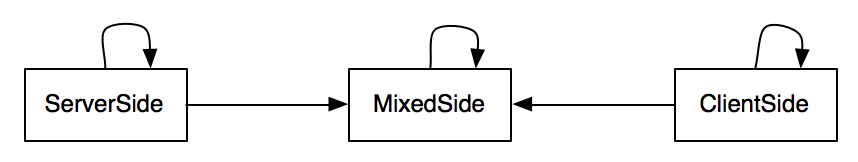
\includegraphics[width=12cm]{resources/images/MixedSidePrinciple.png}}
			\end{center}
			\caption{Visualization of The MixedSide Principle}
			\label{fig:MixedSidePrinciple}
		\end{figure}

		Code annotated with the ClientSide attribute is only meant to be run on client side in form of generated JavaScript. Therefore ClientSide code cannot make calls to methods on, objects that exist only on server side. This would not make sense as server and client side are two different and separated execution contexts.  If client side code were to call server side code, it will ultimately result in a client side error as the server side code will not be mapped to client side. Likewise it will not make sense for server side code to call client side code.

		However mixed side code will both be possible to call from client and server side code. Mixed side code can only consist of C\# constructs that MiCS supports and that MiCS therefore can map to client side code. Furthermore mixed side code can only use other mixed side code and cannot use client side only types such as DOM elements. Because of this it is possible for both server and client side code to call mixed side code.

		All three kinds of code can obviously use other code of the same kind hence the recursive arrows in the illustartion.